\documentclass[12pt,a4paper]{article}

\usepackage[a4paper,margin=1in]{geometry}
\usepackage[T1]{fontenc}
\usepackage[utf8]{inputenc}
\usepackage{lmodern}
\usepackage{setspace}
\usepackage{enumitem}
\usepackage{array}
\usepackage{longtable}
\usepackage{booktabs}
\usepackage{tabularx}
\usepackage{titlesec}
\usepackage[hidelinks]{hyperref}
\usepackage{xcolor}
\usepackage{tikz}
\usetikzlibrary{positioning,shapes.geometric,arrows.meta}

\setstretch{1.12}
\setlength{\parindent}{0pt}
\setlength{\parskip}{6pt}
\titleformat{\section}{\normalfont\large\bfseries}{\thesection}{1em}{}
\titleformat{\subsection}{\normalfont\normalsize\bfseries}{\thesubsection}{1em}{}

\newcolumntype{Y}{>{\raggedright\arraybackslash}X}

\tikzset{
  entity/.style={draw, rectangle, rounded corners=2pt, text width=2.9cm, minimum height=0.9cm, align=center, fill=blue!5, font=\footnotesize},
  rel/.style={draw, diamond, aspect=2, text width=1.8cm, align=center, fill=orange!10, inner sep=1.2pt, font=\footnotesize},
  note/.style={font=\scriptsize, align=center},
  line/.style={-Latex, thick}
}

\begin{document}

\begin{center}
\textbf{UNIVERSITY OF CHITTAGONG}\\
Department of Computer Science and Engineering
\end{center}

\vspace{0.8cm}

\begin{center}
\textbf{\Large Mini-Project Report: Task 2}\\
\textbf{Improved ER Design And Relational Model For A Medical Database}
\end{center}

\vspace{0.8cm}

\textbf{Course Title:} Database Management System\\
\textbf{Course Code:} CSE 414

\vspace{0.8cm}

\textbf{Submitted to:}\\
Dr. Rudra Pratap Deb Nath\\
Professor\\
Department of Computer Science and Engineering\\
University of Chittagong

\vspace{0.8cm}

\textbf{Submitted by:}\\
Name: Sheikh Tawsif Bin Aftab\\
ID: 24701026\\
Session: 2023--2024 B.Sc. Engineering (4th Semester)\\
Department of Computer Science and Engineering\\
University of Chittagong

\vspace{0.8cm}

\textbf{Date of Submission:}\\
10 April 2026

\newpage

\section{Relevant Data Identified}
Based on the sample workbook and the sample query list, the following data items are relevant:

\begin{itemize}[leftmargin=1.5em]
    \item \textbf{Drug:} generic drug name.
    \item \textbf{Drug category:} one drug may belong to multiple categories.
    \item \textbf{Disease:} disease name and its disease category.
    \item \textbf{Side effect:} named adverse effect caused by one or more drugs.
    \item \textbf{Product:} commercial product name for a drug.
    \item \textbf{Company:} manufacturer or marketer of a product.
    \item \textbf{Drug interaction:} symmetric interaction between two drugs.
    \item \textbf{Clinical trial:} title, dates, participant count, and status.
    \item \textbf{Institution:} institution name, country, and address for the trial site.
    \item \textbf{Researcher:} the main researcher responsible for a trial.
    \item \textbf{Condition:} condition explicitly studied in a clinical trial.
\end{itemize}

The sample file strongly suggests that drugs, side effects, treated diseases, products, and trial
conditions are all multi-valued with respect to a single row in the spreadsheet. Therefore, these
must be represented by separate entities and relationship sets rather than repeated columns.

\section{ER Diagram}
To keep the full design readable on a single page, the ER model is shown in two connected parts.
Together, they represent the same medical-database design.

\subsection{Part A: Drug, Disease, Product, And Side-Effect View}
\begin{center}
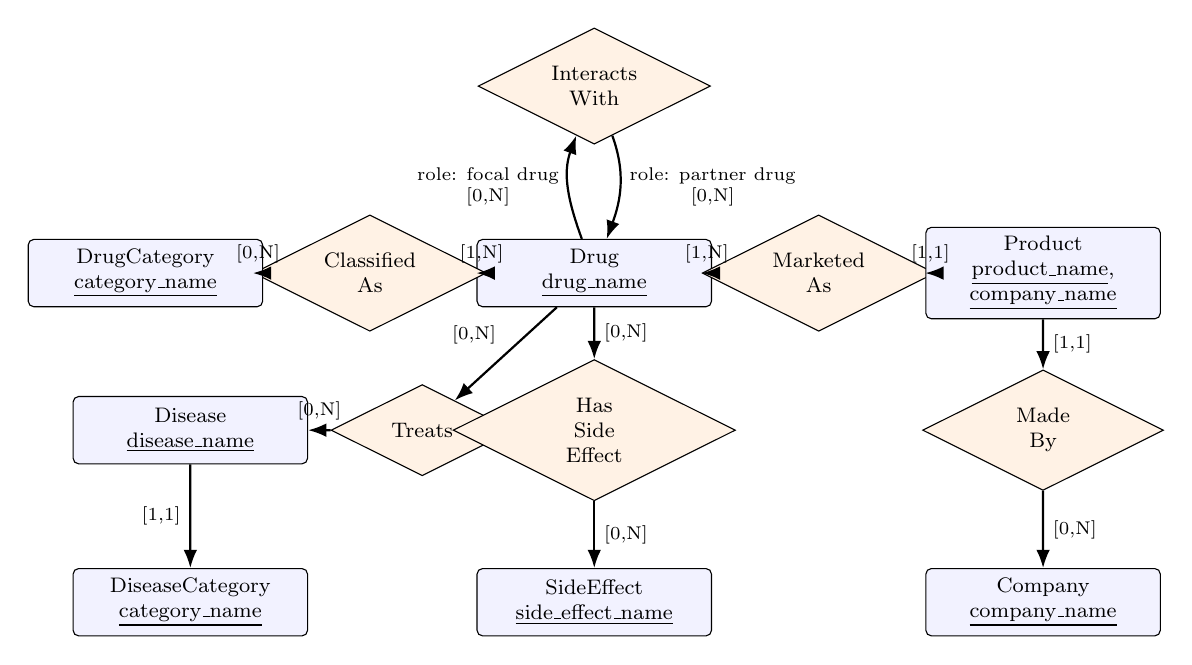
\begin{tikzpicture}[scale=0.95, transform shape]
    \node[entity] (drug) at (0,0) {Drug\\\underline{drug\_name}};
    \node[rel] (classifies) at (-3.0,0) {Classified\\As};
    \node[entity] (drugcat) at (-6.0,0) {DrugCategory\\\underline{category\_name}};

    \node[rel] (interacts) at (0,2.5) {Interacts\\With};

    \node[rel] (treats) at (-2.3,-2.1) {Treats};
    \node[entity] (disease) at (-5.4,-2.1) {Disease\\\underline{disease\_name}};
    \node[entity] (diseasecat) at (-5.4,-4.4) {DiseaseCategory\\\underline{category\_name}};

    \node[rel] (hasse) at (0,-2.1) {Has\\Side\\Effect};
    \node[entity] (sideeffect) at (0,-4.4) {SideEffect\\\underline{side\_effect\_name}};

    \node[rel] (marketed) at (3.0,0) {Marketed\\As};
    \node[entity] (product) at (6.0,0) {Product\\\underline{product\_name},\\\underline{company\_name}};
    \node[rel] (madeby) at (6.0,-2.1) {Made\\By};
    \node[entity] (company) at (6.0,-4.4) {Company\\\underline{company\_name}};

    \draw[line] (drugcat) -- node[note, above] {[0,N]} (classifies);
    \draw[line] (classifies) -- node[note, above] {[1,N]} (drug);

    \draw[line] (drug) -- node[note, above left] {[0,N]} (treats);
    \draw[line] (treats) -- node[note, above] {[0,N]} (disease);
    \draw[line] (disease) -- node[note, left] {[1,1]} (diseasecat);

    \draw[line] (drug) -- node[note, right] {[0,N]} (hasse);
    \draw[line] (hasse) -- node[note, right] {[0,N]} (sideeffect);

    \draw[line] (drug) -- node[note, above] {[1,N]} (marketed);
    \draw[line] (marketed) -- node[note, above] {[1,1]} (product);
    \draw[line] (product) -- node[note, right] {[1,1]} (madeby);
    \draw[line] (madeby) -- node[note, right] {[0,N]} (company);

    \draw[line] (drug) to[out=110,in=250] node[note, left] {role: focal drug\\{}[0,N]} (interacts);
    \draw[line] (interacts) to[out=290,in=70] node[note, right] {role: partner drug\\{}[0,N]} (drug);
\end{tikzpicture}
\end{center}

\subsection{Part B: Clinical-Trial View}
\begin{center}
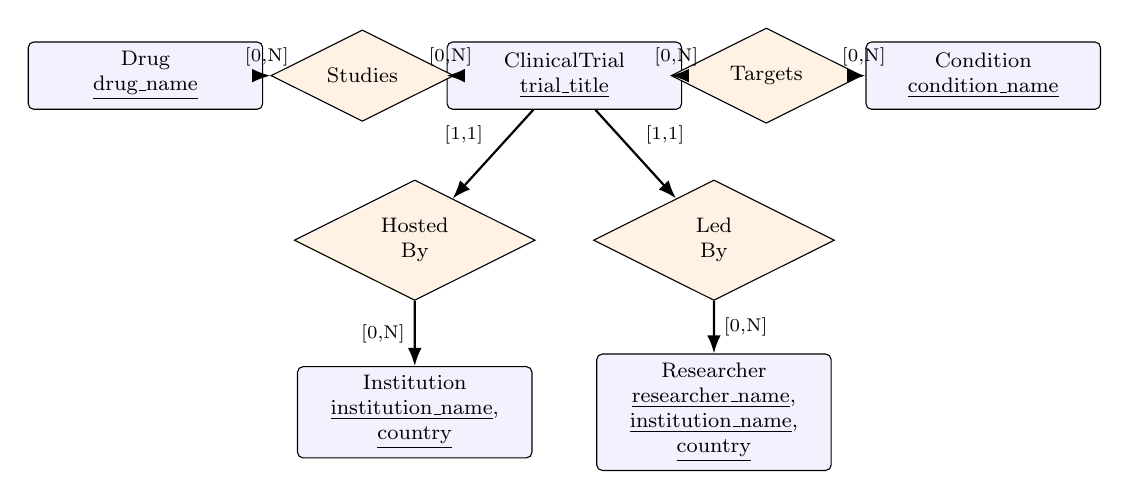
\begin{tikzpicture}[scale=0.95, transform shape]
    \node[entity] (trial) at (0,0) {ClinicalTrial\\\underline{trial\_title}};
    \node[rel] (studies) at (-2.7,0) {Studies};
    \node[entity] (drug) at (-5.6,0) {Drug\\\underline{drug\_name}};

    \node[rel] (targets) at (2.7,0) {Targets};
    \node[entity] (condition) at (5.6,0) {Condition\\\underline{condition\_name}};

    \node[rel] (hosted) at (-2.0,-2.2) {Hosted\\By};
    \node[entity] (institution) at (-2.0,-4.5) {Institution\\\underline{institution\_name},\\\underline{country}};

    \node[rel] (ledby) at (2.0,-2.2) {Led\\By};
    \node[entity] (researcher) at (2.0,-4.5) {Researcher\\\underline{researcher\_name},\\\underline{institution\_name},\\\underline{country}};

    \draw[line] (drug) -- node[note, above] {[0,N]} (studies);
    \draw[line] (studies) -- node[note, above] {[0,N]} (trial);

    \draw[line] (trial) -- node[note, above] {[0,N]} (targets);
    \draw[line] (targets) -- node[note, above] {[0,N]} (condition);

    \draw[line] (trial) -- node[note, above left] {[1,1]} (hosted);
    \draw[line] (hosted) -- node[note, left] {[0,N]} (institution);

    \draw[line] (trial) -- node[note, above right] {[1,1]} (ledby);
    \draw[line] (ledby) -- node[note, right] {[0,N]} (researcher);
\end{tikzpicture}
\end{center}

\subsection{Short Description Of Design Choices}
\begin{enumerate}[leftmargin=1.5em]
    \item \textbf{DrugCategory is many-to-many with Drug.} The sample file shows that a single drug may appear in multiple categories, so a single category attribute would lose information.
    \item \textbf{DrugInteraction is a self-relationship.} This is the natural ER representation because both ends of the relationship are drugs.
    \item \textbf{Product uses a composite natural key.} \texttt{(product\_name, company\_name)} was chosen because the same brand name could theoretically be reused by different companies.
    \item \textbf{Institution and Researcher are separate entities.} This makes it easier to ask trial-based questions about locations and main researchers.
    \item \textbf{Condition is separate from Disease.} Trial conditions in the workbook do not always match the disease names used in the drug-treatment rows, so separating them avoids forced or incorrect matches.
\end{enumerate}

\section{Relational Model}
The improved relational model derived from the ER design is:

\renewcommand{\arraystretch}{1.18}
\begin{longtable}{p{0.28\textwidth} p{0.66\textwidth}}
\toprule
\textbf{Relation} & \textbf{Attributes, keys, and foreign keys} \\
\midrule
\endfirsthead
\toprule
\textbf{Relation} & \textbf{Attributes, keys, and foreign keys} \\
\midrule
\endhead
\texttt{Drug} & \texttt{drug\_name} (PK, CK) \\
\texttt{DrugCategory} & \texttt{category\_name} (PK, CK) \\
\texttt{DrugHasCategory} & \texttt{drug\_name} (PK, FK$\rightarrow$Drug), \texttt{category\_name} (PK, FK$\rightarrow$DrugCategory) \\
\texttt{DiseaseCategory} & \texttt{category\_name} (PK, CK) \\
\texttt{Disease} & \texttt{disease\_name} (PK, CK), \texttt{category\_name} (FK$\rightarrow$DiseaseCategory) \\
\texttt{SideEffect} & \texttt{side\_effect\_name} (PK, CK) \\
\texttt{DrugTreats} & \texttt{drug\_name} (PK, FK$\rightarrow$Drug), \texttt{disease\_name} (PK, FK$\rightarrow$Disease) \\
\texttt{DrugHasSideEffect} & \texttt{drug\_name} (PK, FK$\rightarrow$Drug), \texttt{side\_effect\_name} (PK, FK$\rightarrow$SideEffect) \\
\texttt{DrugInteraction} & \texttt{drug\_name} (PK, FK$\rightarrow$Drug), \texttt{interacting\_drug\_name} (PK, FK$\rightarrow$Drug). A check constraint stores each unordered pair once. \\
\texttt{Company} & \texttt{company\_name} (PK, CK) \\
\texttt{Product} & \texttt{product\_name}, \texttt{company\_name}, \texttt{drug\_name}; PK = \texttt{(product\_name, company\_name)}; FK \texttt{company\_name}$\rightarrow$Company; FK \texttt{drug\_name}$\rightarrow$Drug \\
\texttt{Institution} & \texttt{institution\_name}, \texttt{country}, \texttt{facility\_address}; PK = \texttt{(institution\_name, country)} \\
\texttt{Researcher} & \texttt{researcher\_name}, \texttt{institution\_name}, \texttt{country}; PK = \texttt{(researcher\_name, institution\_name, country)}; FK \texttt{(institution\_name, country)}$\rightarrow$Institution \\
\texttt{ClinicalTrial} & \texttt{trial\_title} (PK, CK), \texttt{start\_date}, \texttt{completion\_date}, \texttt{participants}, \texttt{status}, \texttt{institution\_name}, \texttt{country}, \texttt{main\_researcher\_name}; FK \texttt{(institution\_name, country)}$\rightarrow$Institution; FK \texttt{(main\_researcher\_name, institution\_name, country)}$\rightarrow$Researcher \\
\texttt{ClinicalTrialStudiesDrug} & \texttt{trial\_title} (PK, FK$\rightarrow$ClinicalTrial), \texttt{drug\_name} (PK, FK$\rightarrow$Drug) \\
\texttt{Condition} & \texttt{condition\_name} (PK, CK) \\
\texttt{ClinicalTrialCondition} & \texttt{trial\_title} (PK, FK$\rightarrow$ClinicalTrial), \texttt{condition\_name} (PK, FK$\rightarrow$Condition) \\
\bottomrule
\end{longtable}

The matching SQL version of this improved schema is also stored in:

\texttt{SQL/Medical\_Database/task2\_natural\_key\_schema.sql}

\section{Comparison With Task 1}
Compared with the preliminary Task 1 design, the new design is better in several ways:

\begin{itemize}[leftmargin=1.5em]
    \item \textbf{Natural keys are used more carefully.} In Task 1, most entities used surrogate integer IDs. In Task 2, natural keys are preferred wherever the mini-world provides a stable textual identifier.
    \item \textbf{Cardinalities are explicit.} The Task 2 ER model clearly shows one-to-many and many-to-many relationships using Chen-style relationships and \texttt{[min,max]} constraints.
    \item \textbf{Non-trivial structures are handled more honestly.} Drug categories are modeled as many-to-many, and drug interactions are modeled as a symmetric self-relationship.
    \item \textbf{Clinical-trial information is more precise.} Institution, researcher, studied drug, and studied condition are separated so that advanced trial queries can be answered without ambiguity.
    \item \textbf{The model is closer to course expectations.} The new version is a proper conceptual design and a cleaner relational mapping, not just a collection of tables.
\end{itemize}

These differences occurred because Task 2 uses more database-design knowledge than Task 1. In the
first attempt, the main goal was to break the spreadsheet into usable tables. In the second attempt,
the goal was to produce a more defensible ER design with better key choices, clearer semantics, and
more precise relationship structure.

\section{Conclusion}
The improved Task 2 model captures the medical mini-world more accurately than the preliminary
design. It supports the full set of sample queries, uses course-style ER notation and cardinality
thinking, and provides a relational schema that is cleaner and easier to justify.

\end{document}
